\documentclass[11pt,a4paper]{article}
\usepackage[margin=2.2cm]{geometry}
\usepackage[T1]{fontenc}
\usepackage{charter}
\usepackage{microtype}
\usepackage{graphicx}
\usepackage{booktabs}
\usepackage{array}
\usepackage{tabularx}
\usepackage{float}
\usepackage{caption}
\usepackage{enumitem}
\usepackage{amsmath}
\usepackage[table]{xcolor}
\usepackage{listings}
\usepackage[most]{tcolorbox}
\usepackage{fancyhdr}
\usepackage[colorlinks=true,linkcolor=accent,urlcolor=accent]{hyperref}

\definecolor{accent}{HTML}{3C3489}
\definecolor{codebg}{HTML}{F6F6F3}
\definecolor{kw}{HTML}{185FA5}
\definecolor{cm}{HTML}{6B6A64}
\definecolor{okgreen}{HTML}{0F6E56}
\definecolor{badred}{HTML}{A32D2D}

\setlength{\parindent}{0pt}
\setlength{\parskip}{6pt}
\setlist{itemsep=2pt,topsep=4pt}
\captionsetup{font=small,labelfont=bf}
\renewcommand{\arraystretch}{1.18}

\pagestyle{fancy}\fancyhf{}
\rhead{\small\color{cm}\reporttag}
\cfoot{\small\thepage}
\renewcommand{\headrulewidth}{0.3pt}

\lstdefinelanguage{SV}{
  morekeywords={module,endmodule,input,output,inout,logic,wire,reg,always_ff,always_comb,assign,
    begin,end,if,else,case,endcase,default,typedef,enum,localparam,posedge,negedge,or,task,endtask,
    function,endfunction,automatic,initial,repeat,while,for,integer,string,signed,void},
  sensitive=true, morecomment=[l]{//}, morecomment=[s]{/*}{*/}, morestring=[b]"}
\lstdefinelanguage{ICCTcl}{
  morekeywords={set_app_var,create_mw_lib,open_mw_lib,import_designs,read_sdc,set_tlu_plus_files,
    save_mw_cel,create_floorplan,derive_pg_connection,create_rectangular_ring,create_power_strap,
    create_fp_placement,place_opt,clock_opt,report_placement_utilization,report_qor,report_timing,
    insert_stdcell_filler,route_opt,verify_zrt_route,extract_rc,write_parasitics,write_verilog,
    close_mw_cel,gui_start},
  sensitive=true, morecomment=[l]{\#}}
\lstset{basicstyle=\ttfamily\footnotesize, backgroundcolor=\color{codebg}, frame=single,
  rulecolor=\color{codebg}, keywordstyle=\color{kw}\bfseries, commentstyle=\color{cm}\itshape,
  columns=fullflexible, keepspaces=true, breaklines=true, showstringspaces=false,
  xleftmargin=4pt, xrightmargin=4pt, aboveskip=6pt, belowskip=6pt}

\newtcolorbox{task}{colback=accent!5,colframe=accent,boxrule=0.6pt,arc=2pt,
  left=8pt,right=8pt,top=4pt,bottom=4pt,fonttitle=\bfseries,title=The assignment}
\newtcolorbox{keypoint}[1]{colback=okgreen!6,colframe=okgreen,boxrule=0.6pt,arc=2pt,
  left=8pt,right=8pt,top=4pt,bottom=4pt,fonttitle=\bfseries,title={#1}}
\newtcolorbox{lesson}[1]{colback=orange!7,colframe=orange!70!black,boxrule=0.6pt,arc=2pt,
  left=8pt,right=8pt,top=4pt,bottom=4pt,fonttitle=\bfseries,title={#1}}

\newcommand{\fig}[3]{\begin{figure}[H]\centering\includegraphics[width=#2\linewidth]{figures/#1}\caption{#3}\end{figure}}
\newcommand{\met}{\textcolor{okgreen}{\textbf{MET}}}
\newcommand{\viol}{\textcolor{badred}{\textbf{VIOLATED}}}
% numbers still to be copied from my own .rpt files (shows in red until filled in)
\newcommand{\fillin}[1]{\textcolor{badred}{\textbf{[#1]}}}

\newcommand{\header}[3]{%
  \begin{center}
  {\small\color{cm} CPE 527 VLSI Design \quad|\quad Lab 3 \quad|\quad University of Alabama in Huntsville}\\[8pt]
  {\LARGE\bfseries\color{accent} #1}\\[4pt]
  {\large #2}\\[8pt]
  {\small Bibek Shrestha \quad|\quad October 2026 \quad|\quad #3}
  \end{center}\vspace{2pt}\hrule\vspace{6pt}}
\newcommand{\reporttag}{Lab 3 / Tutorial: gray counter place and route}

\begin{document}
\header{Place and Route of a 4-bit Gray Counter}{From the Lab 2 netlist to a routed layout in IC Compiler}{Synopsys IC Compiler, SAED 90\,nm}

\begin{task}
Take the synthesized gray counter from the previous lab through automatic placement and routing with
IC Compiler: floorplan, power plan, placement, clock tree synthesis and routing. Generate and analyze reports.
\end{task}

\section*{At a glance}
\begin{table}[H]\centering\small
\begin{tabular}{lcc}
\toprule
 & \textbf{After CTS} & \textbf{After routing} \\
\midrule
Clock target & 5 ns & 5 ns \\
Critical path & \fillin{ns} & \fillin{ns} \\
Setup slack & \fillin{ns} & \fillin{ns} \\
Hold violations & \fillin{} & \fillin{} \\
Cells (logic + flip-flops) & \fillin{} & \fillin{} \\
Cell area & \fillin{} & \fillin{} \\
Utilization & \fillin{\%} & \fillin{\%} \\
Net length & \fillin{\textmu m} & \fillin{\textmu m} \\
Open nets / DRCs & & \fillin{} / \fillin{} \\
\bottomrule
\end{tabular}
\caption{Results from my QoR, utilization and \texttt{verify\_zrt\_route} reports.}
\end{table}

\section{The design}
A 4-bit counter that steps through Gray code, so only one bit changes per step:
0, 1, 3, 2, 6, 7, 5, 4, C, D, F, E, A, B, 9, 8, then back to 0.
It has an active-low asynchronous reset \texttt{reset\_n} and an enable \texttt{en\_count}.
The \texttt{case} statement is just a 16-entry next-state table.

\fig{gc_block.png}{0.78}{What the RTL becomes: a 4-bit register with the next-state table in front of it.}

Synthesis mapped my version to 4 \texttt{DFFARX1} flip-flops and 11 logic gates
(\texttt{MUX21X1}, \texttt{XOR2X1}, \texttt{NAND2X0}, \texttt{NOR2X0}, \texttt{AND2X1}, \texttt{INVX0}).
The tutorial's run used \texttt{AO22X1} cells instead of muxes. Same logic, different gate choice.

\fig{gc_wave.png}{0.95}{Expected output for the given testbench (20\,ns clock). Changes made by the testbench on a clock edge are seen one edge later.}

\section{Workflow}
\fig{flow.png}{0.9}{Place and route flow. Each green label is a checkpoint saved in the Milkyway library.}

\begin{enumerate}
\item \textbf{Setup:} point ICC to the SAED90 libraries and create the Milkyway library \texttt{gray4bcntLIB}
      with the technology file and the cell abstracts (FRAM).
\item \textbf{Import} \texttt{gray\_counter.ddc} from Lab 2, read the SDC (5\,ns clock), set the TLU+ wire models.
\item \textbf{Floorplan and power plan}, then a quick \texttt{create\_fp\_placement}.
\item \textbf{Placement and CTS} with \texttt{place\_opt} and \texttt{clock\_opt}, then the first set of reports.
\item \textbf{Fillers and routing} with \texttt{route\_opt}, check with \texttt{verify\_zrt\_route}, second set of reports.
\item \textbf{Extract} parasitics and write the final netlist.
\end{enumerate}

\begin{lstlisting}[language=bash]
cd syn_tut/icc                      # one level below output/ and constraints/
icc_shell -shared_license -f ../src/icc_flow.tcl | tee icc_output.txt
\end{lstlisting}

\section{Floorplan and power plan}
\begin{table}[H]\centering\small
\begin{tabular}{ll}
\toprule
Setting & Value \\
\midrule
Core utilization & 0.6 (cells fill 60\% of the core, the rest is for wiring) \\
Core to die gap & 30\,\textmu m on all four sides \\
VSS ring / VDD ring & 1\,\textmu m wide, offset 0.5 / 1.8\,\textmu m; M6 vertical, M7 horizontal \\
Power straps & VDD and VSS, M6, vertical, 3\,\textmu m wide \\
\bottomrule
\end{tabular}
\caption{Floorplan settings (same as the tutorial).}
\end{table}

\begin{figure}[H]\centering
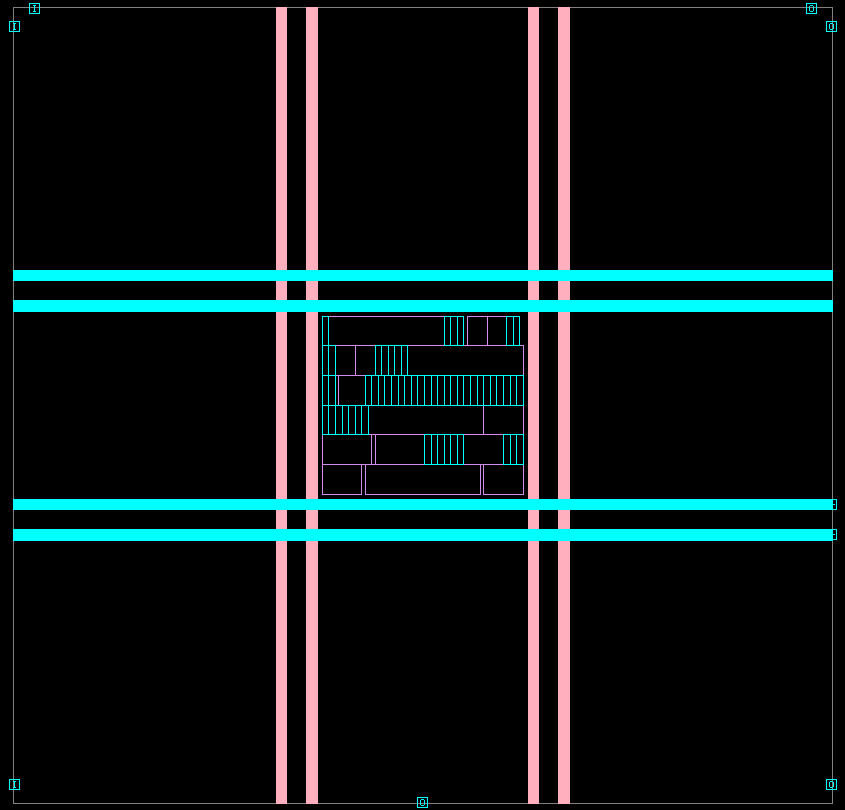
\includegraphics[width=0.48\linewidth]{figures/icc_fp_placement.png}
\caption{After \texttt{create\_fp\_placement}: rings (cyan), straps (pink) and the cells placed in rows in the middle.}
\end{figure}

\section{Placement, clock tree and routing}
\texttt{place\_opt} legalized the cells and checked timing. \texttt{clock\_opt} built the clock network to
the 4 flip-flops. Fillers (\texttt{SHFILL2}) closed the gaps in the rows so the power rails run unbroken,
and \texttt{route\_opt} drew the signal wires.

\fig{icc_routed.png}{0.72}{Zoom on the routed block. Labels are my cell instances; pink and violet are routed metal.}

\section{Reports}
\begin{table}[H]\centering\small
\begin{tabular}{lll}
\toprule
Report & What I checked & Result \\
\midrule
\texttt{*\_qor.rpt} & slack, violating paths & \fillin{} \\
\texttt{*.setup.rpt} & worst setup path & \fillin{start $\rightarrow$ end, slack} \\
\texttt{*.hold.rpt} & worst hold path & \fillin{} \\
\texttt{*\_util.rpt} & standard cell utilization & \fillin{} \\
\texttt{verify\_zrt\_route} & open nets, DRCs & \fillin{} \\
\bottomrule
\end{tabular}
\caption{What each report says for my run.}
\end{table}

\section{Inside the cells}
ICC places and routes with the abstract (FRAM) view of each cell: only the outline, the pins and the
blocked metal. The full layout (CEL view) has every mask layer.

\begin{figure}[H]\centering
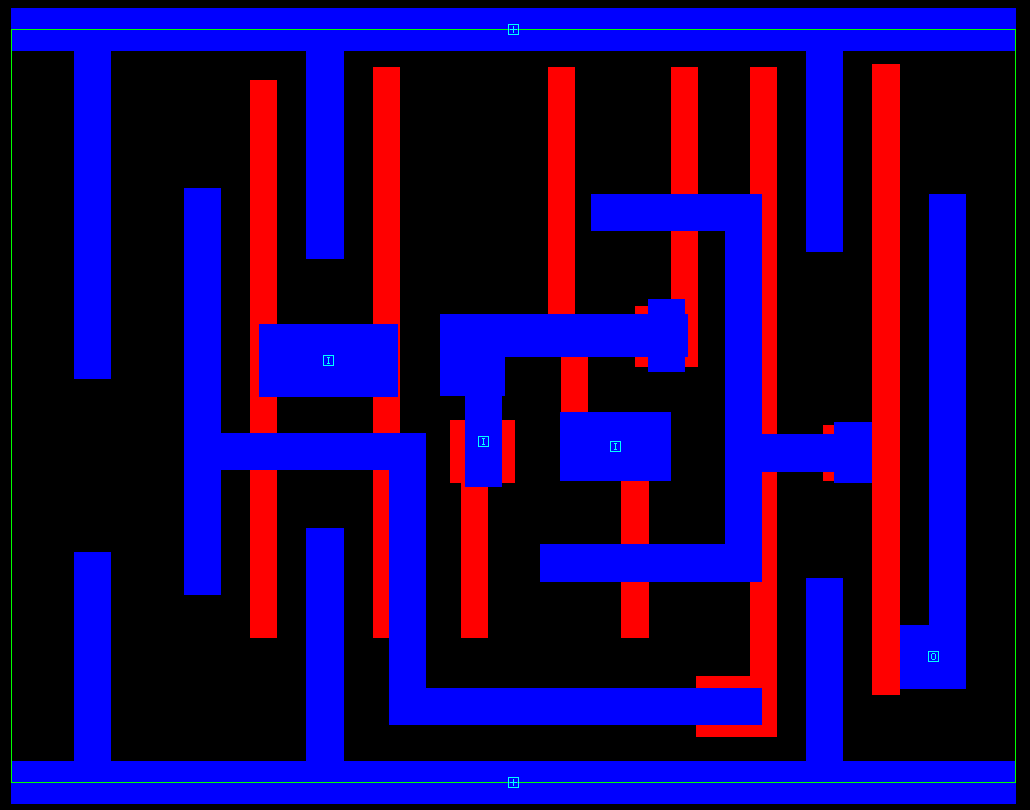
\includegraphics[height=5.6cm]{figures/icc_mux21x1_fram.png}\hfill
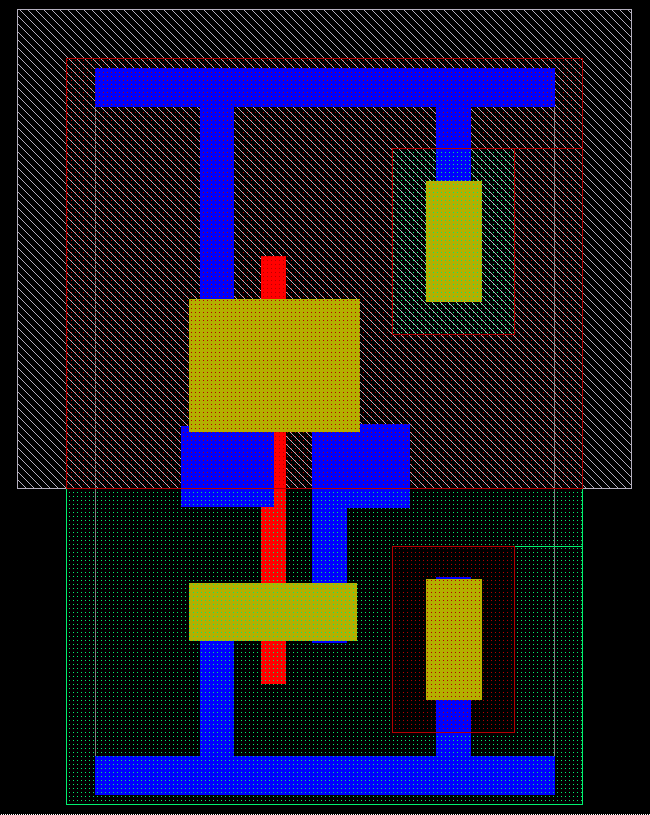
\includegraphics[height=5.6cm]{figures/icc_invx0_cel.png}
\caption{Left: \texttt{MUX21X1} FRAM view, with VDD/VSS rails at top and bottom and the pin squares in between.
Right: \texttt{INVX0} CEL view. PMOS sits in the N-well (hatched, top), NMOS below, and one poly gate (red) drives both.}
\end{figure}

\section{What I learned}
\begin{itemize}
\item Physical design starts from the synthesized \texttt{.ddc}, so the gates are already fixed; ICC only decides where they go and how they connect.
\item Utilization is a trade-off: a smaller core saves area but leaves less room to route.
\item The power grid (rings, straps, cell rails) is built before any cell is placed.
\item The \texttt{PATH} in the tutorial did not exist on our server. ICC is installed at
\begin{lstlisting}[language=bash]
/apps/synopsys2023/icc/V-2023.12-SP5/bin
\end{lstlisting}
\item \texttt{create\_mw\_lib} runs only once. After that, use \texttt{open\_mw\_lib}.
\end{itemize}

\appendix
\section{Source files}
\subsection*{RTL: \texttt{src/gray\_counter.sv}}
\lstinputlisting[language=SV]{src/gray_counter.sv}
\subsection*{Testbench: \texttt{src/gray\_counter\_tb.sv}}
\lstinputlisting[language=SV]{src/gray_counter_tb.sv}
\subsection*{ICC script: \texttt{src/icc\_flow.tcl}}
\lstinputlisting[language=ICCTcl]{src/icc_flow.tcl}
\end{document}
